% =====================================================================
%  Презентация для конференции «Научный Телеграф» 2026
%  Команда MusicTech, Центральный Университет (Т-Банк)
%
%  Стиль: фирменный beamer команды (Madrid + seahorse, pdflatex).
%  Согласован со статьёй (article/main.tex) и тезисами
%  (article/тезисы.tex). Без \pause, по плану PRESENTATION.md.
%
%  Сборка:  pdflatex presentation.tex × 2
%  Либо:    .\build.ps1
% =====================================================================
\documentclass[10pt]{beamer}

\usetheme{Madrid}
\usecolortheme{seahorse}

\usepackage[T2A]{fontenc}
\usepackage[utf8]{inputenc}
\usepackage[russian]{babel}
\usepackage{graphicx}
\usepackage{xcolor}
\usepackage{tikz}
\usetikzlibrary{
  arrows.meta, positioning, fit, calc, shapes.geometric,
  shapes.misc, decorations.pathreplacing, decorations.markings,
  patterns, backgrounds, matrix, intersections
}
\usepackage{pgfplots}
\pgfplotsset{compat=1.18}
\usepackage{amsmath, amssymb, mathtools}
\usepackage{booktabs}
\usepackage{listings}

% Лёгкая подсветка ключевых слов (синий — акцент seahorse-палитры)
\definecolor{accentblue}{HTML}{2581C4}
\newcommand{\rlhi}[1]{{\color{accentblue}\textbf{#1}}}

% Подпись под графиком / схемой
\newcommand{\figcaption}[1]{%
  {\par\vspace{0.3em}\footnotesize\itshape\color{black!75}#1\par}%
}

\DeclareMathOperator*{\argmin}{arg\,min}
\DeclareMathOperator*{\argmax}{arg\,max}
\providecommand{\Real}{\mathbb{R}}
\providecommand{\Expect}{\mathbb{E}}

% Listings под JSON
\lstdefinestyle{json}{
  basicstyle=\ttfamily\footnotesize,
  numbers=none,
  showstringspaces=false,
  breaklines=true,
  frame=single,
  rulecolor=\color{accentblue},
  keywordstyle=\color{accentblue}\bfseries,
  stringstyle=\color{black!70},
  morekeywords={true, false, null},
}
\lstset{style=json}

% Пути к графике
\graphicspath{{figures/}{figures/png/}{figures/generated/}{figures/tikz/}}

\title[Адаптивный аккомпанемент в реальном времени]{%
  Адаптивный аккомпанемент в реальном времени:\\
  от классических трекеров партитуры\\
  к RL-агенту опережающего темпа}
\author[Новицкий, Борисов, Варламов]{Н.~И. Новицкий \and Н.~С. Борисов \and А.~А. Варламов}
\institute[ЦУ]{АНО Центральный Университет, мастерская MusicTech}
\date{Научный Телеграф, 2026}

\logo{
\includegraphics[height=0.8cm]{cu_logo.png}}

\begin{document}

% =========================================================
\begin{frame}
  \titlepage
\end{frame}

\begin{frame}{Структура презентации}
  \tableofcontents
\end{frame}

% =========================================================
\section{Введение}
% =====================================================================
% Введение (по стилю HW_10_PRESENTATION_NP.tex)
% =====================================================================
\begin{frame}{Введение}

\textbf{Актуальность:} солисты-пианисты при подготовке к концерту
нуждаются в репетициях с оркестровым сопровождением, однако живой
оркестр недоступен на каждой репетиции. Фиксированная фонограмма не
подстраивается под темп и \emph{rubato} солиста.

\bigskip

\textbf{Проблема:} построить виртуальный оркестр, который в реальном
времени отслеживает позицию исполнителя в партитуре и упреждающе
управляет темпом аккомпанемента (бюджет задержки $\le 20$\,мс ---
порог восприятия рассинхронизации в ансамбле, Cont 2010).

\bigskip

\textbf{Подход:} классический трекер партитуры (HMM\,$+$\,OLTW)
$+$ \emph{лёгкий RL-агент}, который видит состояние трекера и
управляет темпом на горизонте 200--500\,мс.

\bigskip

\textbf{Цель доклада:} разобрать математическую часть baseline,
обосновать формулу награды RL-агента и положение работы относительно
литературы.

\end{frame}


% =========================================================
\section{Постановка задачи}
% =====================================================================
% Слайд 2 — Проблема
% =====================================================================
\begin{frame}{Проблема: аккомпаниатор, а не фонограмма}
  \small
  \begin{columns}[T,onlytextwidth]
    \column{0.46\textwidth}
    \vspace{0.4em}
    \begin{itemize}\setlength{\itemsep}{0.45em}
      \item Солисту-пианисту перед концертом нужно репетировать
            \textbf{с оркестром}.
      \item Живой оркестр на каждую репетицию --- недоступно
            (бюджет, время, организация).
      \item Фиксированная фонограмма не работает: она не
            подстраивается под темп, артикуляцию и \emph{rubato}
            солиста.
      \item \rlhi{Цель:} виртуальный оркестр, который играет
            заданное сопровождение и подстраивается под солиста
            \textbf{в реальном времени}.
    \end{itemize}

    \column{0.54\textwidth}
    \centering
    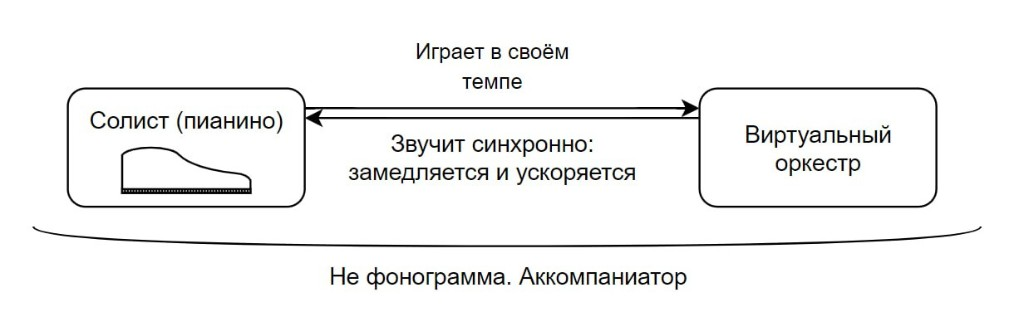
\includegraphics[width=\linewidth]{figures/png/world_view.png}
  \end{columns}
\end{frame}

% =====================================================================
% Слайд 3 — Что технически делает система
% =====================================================================
\begin{frame}{Что технически делает система}
  \small
  Задача формализуется как \rlhi{score-following}: по поступающему
  MIDI/аудио-потоку и заранее известной партитуре в реальном времени
  определять текущую позицию исполнителя.

  \begin{columns}[T,onlytextwidth]
    \column{0.42\textwidth}
    \begin{itemize}\setlength{\itemsep}{0.4em}
      \item \textbf{Вход:} партитура (известна) + поток нот солиста
            (realtime).
      \item \textbf{Выход:} индекс ноты $\hat\imath_t$
            $+$ темповый коэффициент $\tau_t$.
      \item \textbf{Бюджет задержки:} $\le 20$ мс
            (порог восприятия рассинхронизации, Cont 2010).
    \end{itemize}

    \column{0.58\textwidth}
    \centering
    % СХЕМА 2 — Pipeline системы (вход → Core ML → выход + RL на боку)
\begin{tikzpicture}[
  every node/.style={font=\footnotesize, align=center},
  box/.style={draw, thick, minimum height=0.9cm, minimum width=1.5cm,
              rounded corners=1.5pt, fill=white, inner sep=2pt},
  small/.style={font=\scriptsize},
  arr/.style={-{Latex[length=2mm]}, thick},
]
  \node[box]                            (in)   {MIDI /\\микрофон};
  \node[box, right=0.4cm of in]         (sf)   {Score\\follower};
  \node[box, right=0.4cm of sf]         (tt)   {Tempo\\Tracker};
  \node[box, right=0.4cm of tt]         (rend) {Renderer};
  \node[box, right=0.4cm of rend]       (out)  {Звуковая\\карта};

  \draw[arr] (in)   -- (sf);
  \draw[arr] (sf)   -- node[above, small] {$\hat\imath_t$} (tt);
  \draw[arr] (tt)   -- node[above, small] {$\tau_t$} (rend);
  \draw[arr] (rend) -- (out);

  % Bracket: Core ML over sf + tt
  \draw[decorate, decoration={brace, amplitude=4pt, raise=2pt}]
        ($(sf.north west) + (0,0.05)$) --
        ($(tt.north east) + (0,0.05)$)
        node[midway, above=8pt, small] {\itshape Core ML};

  % RL agent (dashed, off to the side)
  \node[box, dashed, below=1.1cm of tt, fill=black!4] (rl)
        {\bfseries RL-агент\\\scriptsize\itshape (план)};
  \draw[arr, dashed] (rl) -- (tt);
  \node[small, right=1pt of rl, anchor=west, text width=4cm]
        {\itshape опережающее\\предсказание темпа\\на 200--500 мс};
\end{tikzpicture}

    \figcaption{Core ML (HMM/HSMM/OLTW) и TempoTracker --- классическое
             ядро. RL-агент \emph{дополняет} ядро опережающим
             предсказанием темпа на 200--500 мс.}
  \end{columns}
\end{frame}



% =========================================================
\section{Данные: партитура и исполнение}
% =====================================================================
% Слайд 4 — Данные: формат партитуры
% =====================================================================
\begin{frame}[fragile]{Данные: формат партитуры}
  \small
  Партитура хранится в JSON-формате \texttt{score.json}. Одна запись
  $=$ одно скрытое состояние HMM/HSMM (может быть аккордом).

  \begin{columns}[T,onlytextwidth]
    \column{0.45\textwidth}
\begin{verbatim}
{
  "index": 0,
  "pitches": [60, 64, 67],
  "nominal_onset":    2.999,
  "nominal_duration": 1.499
}
\end{verbatim}
    \begin{itemize}\footnotesize
      \item \texttt{generated\_dataset/} --- 4 синтетические пары;
      \item \texttt{midi/library/rach\_solo/} --- Рахманинов,
            \textbf{3791 state};
      \item для RL --- импортер ASAP (Foscarin 2020): 222 пьесы,
            1067 исполнений с note-level разметкой.
    \end{itemize}

    \column{0.55\textwidth}
    \centering
    % ГРАФИК 1 — Pitch vs time для rach_solo (схематически, ч/б).
% Данные сгенерированы как репрезентативная выборка из 3791 state
% Рахманинова — диапазон pitch 28-90, плотный кластер 50-80.
\begin{tikzpicture}
  \begin{axis}[
    width=6cm, height=4.5cm,
    xlabel={Время, c},
    ylabel={MIDI pitch},
    xmin=0, xmax=420,
    ymin=28, ymax=92,
    tick style={black},
    axis line style={black},
    grid=both,
    grid style={dotted, gray!50},
    label style={font=\footnotesize},
    tick label style={font=\scriptsize},
    title style={font=\footnotesize\itshape},
    title={Рахманинов: 3791 state партитуры}
  ]
    % Scatter point cloud — pseudo-distributed pitches
    \addplot+[
      only marks, mark=*, mark size=0.25pt,
      color=black, opacity=0.55,
    ] table[row sep=\\] {
      x y \\
      5  72\\  6 70\\  8 68\\ 10 65\\ 12 60\\ 14 64\\ 16 67\\ 18 72\\
      22 75\\ 24 79\\ 27 76\\ 30 72\\ 33 67\\ 36 64\\ 40 60\\ 43 64\\
      46 67\\ 49 70\\ 53 73\\ 57 76\\ 60 79\\ 63 75\\ 67 71\\ 71 67\\
      75 63\\ 79 59\\ 84 55\\ 88 51\\ 92 47\\ 96 51\\100 55\\104 60\\
     109 64\\114 68\\118 72\\123 75\\128 78\\133 75\\138 72\\143 68\\
     148 65\\153 60\\158 58\\163 55\\168 52\\172 48\\177 44\\181 41\\
     185 38\\189 44\\194 50\\199 55\\204 60\\209 65\\214 70\\220 75\\
     225 78\\230 80\\235 76\\240 72\\245 68\\250 64\\256 60\\262 56\\
     268 52\\274 56\\280 60\\286 65\\292 70\\298 74\\304 78\\310 81\\
     316 77\\322 73\\328 69\\335 65\\341 60\\347 56\\353 52\\359 48\\
     365 44\\372 49\\378 55\\384 60\\390 66\\396 71\\402 76\\408 80\\
      19 55\\ 21 58\\ 35 50\\ 38 56\\ 52 70\\ 56 64\\ 70 58\\ 80 64\\
      90 70\\ 99 64\\105 70\\110 76\\116 64\\125 66\\135 58\\150 70\\
     160 64\\180 80\\190 72\\200 68\\210 76\\230 88\\240 80\\260 72\\
     280 84\\300 76\\320 64\\340 72\\360 66\\380 75\\400 70\\
      15 36\\ 25 40\\ 35 44\\ 50 36\\ 80 40\\110 36\\140 32\\170 36\\
     200 40\\240 36\\280 32\\320 36\\360 40\\410 36\\
      11 80\\ 18 84\\ 33 88\\ 60 82\\ 95 90\\150 86\\200 88\\280 90\\
     350 84\\
    };
  \end{axis}
\end{tikzpicture}

    \figcaption{Рахманинов, 1-я часть концерта №\,2. Каждая точка~---
             состояние партитуры (верхняя нота аккорда).}
  \end{columns}
\end{frame}


% =====================================================================
% Слайд 5 — Данные: исполнение в реальном времени
% =====================================================================
\begin{frame}[fragile]{Данные: исполнение в реальном времени}
  \small
  Live-поток от солиста --- последовательность MIDI-событий:
\begin{verbatim}
{"pitch": 64, "timestamp": 1.234, "velocity": 88}
{"pitch": 67, "timestamp": 1.481, "velocity": 95}
...
\end{verbatim}

  \begin{columns}[T,onlytextwidth]
    \column{0.40\textwidth}
    \vspace{0.3em}
    В реальном исполнении \texttt{timestamps} \emph{не совпадают} с
    \texttt{nominal\_onset} из-за rubato, ускорений, замедлений и
    ошибок.

    \vspace{0.5em}
    Это и есть \rlhi{challenge задачи}: трекер должен оставаться
    синхронным, даже когда времени между нотами на лету меняется
    в 2--3 раза.

    \column{0.60\textwidth}
    \centering
    % ГРАФИК 2 — Bar-plot rubato deviations (performance_time − score_onset)
\begin{tikzpicture}
  \begin{axis}[
    width=7.5cm, height=4.5cm,
    ybar,
    bar width=4pt,
    xlabel={\# ноты в партитуре},
    ylabel={$t^{\text{perf}} - t^{\text{nom}}$, c},
    xmin=0, xmax=21,
    ymin=-0.45, ymax=0.45,
    tick style={black},
    axis line style={black},
    grid=major,
    grid style={dotted, gray!50},
    xtick={0,5,10,15,20},
    label style={font=\footnotesize},
    tick label style={font=\scriptsize},
    title style={font=\footnotesize\itshape},
    title={Synthetic rubato: ускорение $\to$ замедление}
  ]
    \addplot[
      fill=black!40,
      draw=black,
    ] coordinates {
      (1, -0.05) (2, -0.12) (3, -0.18) (4, -0.22) (5, -0.28)
      (6, -0.30) (7, -0.28) (8, -0.22) (9, -0.15) (10, -0.08)
      (11, 0.02) (12, 0.10) (13, 0.16) (14, 0.21) (15, 0.27)
      (16, 0.32) (17, 0.36) (18, 0.34) (19, 0.28) (20, 0.20)
    };
    \draw[thick] (axis cs:0,0) -- (axis cs:21,0);
  \end{axis}
\end{tikzpicture}

    \figcaption{Типичный rubato: пианист сначала ускоряется
             (отрицательные дельты), потом замедляется
             (положительные). Это паттерн классического исполнения.}
  \end{columns}
\end{frame}



% =========================================================
\section{Классические трекеры (baseline)}
% =====================================================================
% DTW: вывод рекуррентного соотношения (фундамент OLTW)
% =====================================================================
\begin{frame}{Dynamic Time Warping --- основа OLTW (определение)}

\textbf{Дано:} партитура $P = (p_1, p_2, \ldots, p_N)$ (последовательность
pitch-ов) и наблюдаемое исполнение $O = (o_1, o_2, \ldots, o_T)$.

\bigskip

\textbf{Ищем} \emph{warping path} $\pi = ((i_1, t_1), \ldots, (i_L, t_L))$
с тремя свойствами:

\begin{enumerate}
\item граничные условия: $(i_1, t_1) = (1, 1)$, $(i_L, t_L) = (N, T)$;
\item монотонность: $i_{\ell+1} \ge i_\ell$ и $t_{\ell+1} \ge t_\ell$;
\item шаг-1: $(i_{\ell+1} - i_\ell, t_{\ell+1} - t_\ell) \in \{(0,1),(1,0),(1,1)\}$.
\end{enumerate}

\bigskip

\textbf{Стоимость пути}:
\[
\mathrm{cost}(\pi) \;=\; \sum_{\ell=1}^{L} c(p_{i_\ell}, o_{t_\ell}),
\qquad
c(p, o) = |p - o| \text{ (полутоны)}.
\]

\bigskip

\textbf{Оптимальный путь} $\pi^* = \argmin_{\pi} \mathrm{cost}(\pi)$.

\end{frame}

\begin{frame}{DTW --- рекуррентное соотношение (вывод)}

Обозначим $D[i, t]$ --- минимальная стоимость пути из $(1,1)$ в $(i, t)$.

\bigskip

\textbf{Идея вывода:} последний шаг пути приходит в $(i, t)$ из одного
из трёх предков (свойство шаг-1):

\begin{itemize}
  \item диагональ $(i{-}1, t{-}1) \to (i, t)$;
  \item горизонталь $(i{-}1, t) \to (i, t)$;
  \item вертикаль $(i, t{-}1) \to (i, t)$.
\end{itemize}

\bigskip

\textbf{Принцип оптимальности Беллмана:} путь до $(i, t)$ оптимален
$\Longleftrightarrow$ путь до предыдущего шага оптимален. Отсюда:

\[
\boxed{\;
D[i, t] \;=\; c(p_i, o_t) \;+\;
\min\!\Bigl(D[i{-}1, t{-}1],\; D[i{-}1, t],\; D[i, t{-}1]\Bigr)\;}
\]

с базовым случаем $D[1,1] = c(p_1, o_1)$ и $D[\cdot, \cdot] = +\infty$
вне сетки.

\bigskip

\textbf{Сложность:} $O(NT)$ по памяти и времени.

\textbf{Online-проблема:} в realtime $T$ растёт, нельзя хранить весь
массив. \rlhi{Решение --- OLTW.}

\end{frame}

% =====================================================================
% Слайд 6 — Baseline 1: OLTW (наработка лаборатории)
% =====================================================================
\begin{frame}{Baseline 1: OLTW \small(Dixon 2005)}
  \small\setlength{\abovedisplayskip}{2pt}
  \setlength{\belowdisplayskip}{2pt}

  \textbf{On-Line Time Warping} --- инкрементальный вариант DTW.

  \begin{columns}[T,onlytextwidth]
    \column{0.52\textwidth}
    \begin{itemize}\setlength{\itemsep}{0.25em}
      \item Локальная стоимость:
            $\displaystyle c(i,t) = |\,p_i - o_t|$.
      \item Рекурсия:\\
            $\displaystyle D[i,t] = c(i,t) +
             \min\bigl(D[i{-}1,t{-}1],\, D[i{-}1,t],\, D[i,t{-}1]\bigr)$.
      \item Предсказание: $\hat\imath_t = \argmin_i D[i,t]$.
      \item Память $O(N)$ --- хранятся только две колонки.
      \item Монотонизация $+$ \emph{RunCount} fail-safe: если позиция
            $k$ событий не двигается, форсируем шаг вперёд.
    \end{itemize}

    \column{0.48\textwidth}
    \centering
    % СХЕМА 3 — OLTW dynamic programming
\begin{tikzpicture}[
  every node/.style={font=\footnotesize},
  cell/.style={draw, thick, minimum width=1.1cm, minimum height=0.7cm,
               inner sep=1pt, fill=white},
  arr/.style={-{Latex[length=2mm]}},
]
  % Header
  \node[font=\scriptsize] at (0, 3.0) {$t{-}1$};
  \node[font=\scriptsize] at (1.6, 3.0) {$t$};

  % Grid: rows i = 0..4
  \foreach \r/\i in {0/4, 1/3, 2/2, 3/1, 4/0} {
    \node[cell] (p\i) at (0, 2.5-\r*0.75) {$D[\i,t{-}1]$};
    \node[cell] (c\i) at (1.6, 2.5-\r*0.75) {$D[\i,t]$};
    \node[font=\scriptsize] at (-0.95, 2.5-\r*0.75) {$i{=}\i$};
  }

  % Arrows into c2 (D[2,t])
  \draw[arr] (p1) -- (c2);     % diagonal D[i-1,t-1]
  \draw[arr] (p2) -- (c2);     % horizontal D[i,t-1]
  \draw[arr] (c1) -- (c2);     % vertical D[i-1,t]
  \node[font=\scriptsize, right=4pt of p1, anchor=west] {\itshape diag};
  \node[font=\scriptsize, right=4pt of p2, anchor=west] {\itshape horiz};
  \node[font=\scriptsize, right=4pt of c1, anchor=west, xshift=8pt] {\itshape vert};

  % Highlight target cell
  \draw[very thick] (c2.south west) rectangle (c2.north east);

  % Equation below
  \node[align=left, font=\scriptsize] at (1.0, -1.0)
       {$D[i,t] \;=\; c(i,t) \;+\; \min\bigl(D[i{-}1,t{-}1],\; D[i{-}1,t],\; D[i,t{-}1]\bigr)$};
  \node[align=center, font=\scriptsize\itshape] at (1.0, -1.55)
       {Predicted index $= \arg\min_i D[i,t]$};
\end{tikzpicture}

    \figcaption{Predicted index $=$ argmin по текущему столбцу.}
  \end{columns}

  \vspace{0.3em}
  {\footnotesize \textbf{Плюсы:} простота, устойчивость к rubato,
   всегда выдаёт ответ.\quad
   \textbf{Минусы:} нет confidence, плохо ловит структурные ошибки.}
\end{frame}


% =====================================================================
% OLTW: численный пример заполнения двух колонок
% =====================================================================
\begin{frame}{OLTW: численный пример заполнения DP-таблицы}

\textbf{Партитура:} 5 нот гаммы C-мажор $P = (60, 62, 64, 65, 67)$.

\textbf{Поток:} играем первые 4 ноты ровно $O = (60, 62, 64, 65)$.

\textbf{Стоимость:} $c(p_i, o_t) = |p_i - o_t|$ (полутоны).

\bigskip

\textbf{Шаг $t=1$, $o_1 = 60$:}
\[
\begin{array}{c|ccccc}
i & 1 & 2 & 3 & 4 & 5 \\
\hline
p_i & 60 & 62 & 64 & 65 & 67 \\
c(p_i, o_1) & 0 & 2 & 4 & 5 & 7 \\
D[i, 1]     & 0 & 2 & 6 & 11 & 18 \\
\end{array}
\]

(Кумулятивная сумма --- это «вертикальный» шаг $D[i,1] = c(p_i, o_1) + D[i{-}1, 1]$.)

\bigskip

\textbf{Предсказание:} $\hat\imath_1 = \argmin_i D[i, 1] = \rlhi{1}$
(первая нота). 

\end{frame}

\begin{frame}{OLTW: пример заполнения (продолжение)}

\textbf{Шаг $t=2$, $o_2 = 62$.} По рекурсии
$D[i,t] = c(p_i, o_t) + \min(D[i{-}1, t{-}1], D[i{-}1, t], D[i, t{-}1])$:

\[
\begin{array}{c|ccccc}
i & 1 & 2 & 3 & 4 & 5 \\
\hline
c(p_i, o_2) & 2 & 0 & 2 & 3 & 5 \\
D[i, 2]     & 2 & 0 & 2 & 5 & 10 \\
\end{array}
\]

\textbf{Предсказание:} $\hat\imath_2 = \argmin_i D[i, 2] = \rlhi{2}$. 

\bigskip

\textbf{Шаг $t=3$, $o_3 = 64$:}
\[
\begin{array}{c|ccccc}
i & 1 & 2 & 3 & 4 & 5 \\
\hline
c(p_i, o_3) & 4 & 2 & 0 & 1 & 3 \\
D[i, 3]     & 6 & 2 & 0 & 1 & 4 \\
\end{array}
\]
$\hat\imath_3 = \rlhi{3}$.

\bigskip

\textbf{Шаг $t=4$, $o_4 = 65$:} $\hat\imath_4 = \rlhi{4}$
(минимум в строке $i=4$).

\bigskip

\textbf{Итог:} OLTW идеально отслеживает $\hat\imath_t = 1, 2, 3, 4$ ---
ровно по диагонали DP-сетки.\quad
\textbf{Память:} хранилось всего 2 колонки.

\end{frame}

% =====================================================================
% Слайд 7 — Baseline 2: HMM (наработка лаборатории)
% =====================================================================
\begin{frame}{Baseline 2: HMM \small(Rabiner 1989)}
  \footnotesize\setlength{\abovedisplayskip}{3pt}
  \setlength{\belowdisplayskip}{3pt}

  Скрытая Марковская модель по партитуре.

  \begin{columns}[T,onlytextwidth]
    \column{0.50\textwidth}
    \vspace{0.4em}
    \begin{itemize}\setlength{\itemsep}{0.35em}
      \item Состояния: $i \in \{0,\ldots,N{-}1\}$ --- индексы нот.
      \item Эмиссия (гауссиана по pitch, $\sigma$ в полутонах):
            \[
              b_i(o) = \frac{1}{\sigma\sqrt{2\pi}}
              \exp\!\Bigl(-\tfrac12
              \bigl(\tfrac{o - p_i}{\sigma}\bigr)^{\!2}\Bigr)
            \]
      \item Переходы $\{$stay$=0.3$, advance$=0.6$, skip$=0.1\}$,
            веса зависят от \texttt{elapsed} в state.
      \item Forward-обновление:
            \[
              \alpha_{t+1}(i) = b_i(o_{t+1}) \sum_j \alpha_t(j)\, a_{j,i}
            \]
      \item $\hat\imath_t = \argmax_i \alpha_t(i)$,\quad
            \emph{confidence} $= \max_i \alpha_t(i)$.
    \end{itemize}

    \column{0.50\textwidth}
    \centering
    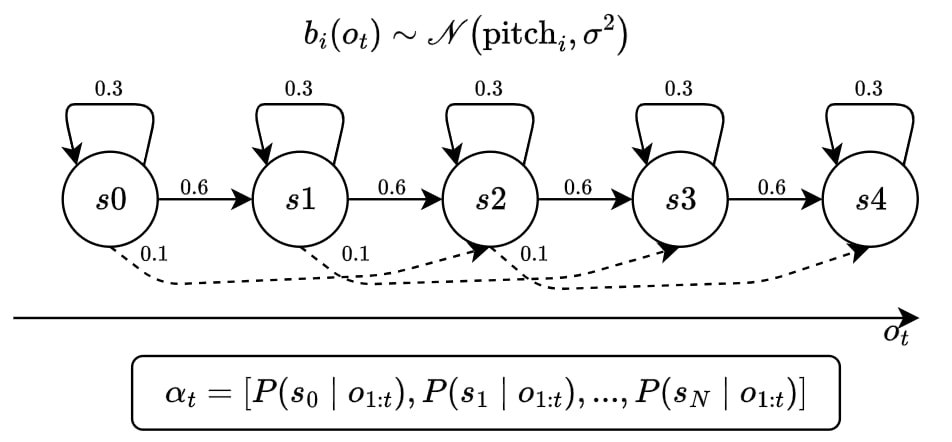
\includegraphics[width=\linewidth]{figures/png/hmm_chain.png}
  \end{columns}
\end{frame}

% =====================================================================
% HMM: вывод Forward-формулы
% =====================================================================
\begin{frame}{HMM: вывод Forward-формулы (Rabiner 1989)}

\textbf{Определим} $\alpha_t(i) = P(O_{1:t},\, S_t = i \mid \lambda)$
--- вероятность, что мы наблюдали $o_1, \ldots, o_t$ и сейчас находимся
в состоянии $i$.

\bigskip

\textbf{Инициализация} (по определению совместного):
\[
\alpha_1(i) \;=\; \pi_i\, b_i(o_1),
\quad i \in \{1, \ldots, N\},
\]
где $\pi_i = P(S_1 = i)$ --- начальное распределение,
$b_i(o) = P(o \mid S=i)$ --- функция эмиссии.

\bigskip

\textbf{Индукция $t \to t+1$:} маргинализуем по предыдущему состоянию
$S_t = j$:
\[
\alpha_{t+1}(i)
\;=\; P(O_{1:t+1},\, S_{t+1}=i)
\;=\; \sum_{j=1}^{N} P(O_{1:t+1},\, S_t = j,\, S_{t+1} = i).
\]

\end{frame}

\begin{frame}{HMM: вывод Forward-формулы (продолжение)}

\textbf{Цепной разбор} по правилу произведения и марковскому свойству:
\[
P(O_{1:t+1}, S_t=j, S_{t+1}=i)
= \underbrace{P(O_{1:t}, S_t=j)}_{=\alpha_t(j)}\;
  \underbrace{P(S_{t+1}=i \mid S_t=j)}_{=a_{j,i}}\;
  \underbrace{P(o_{t+1} \mid S_{t+1}=i)}_{=b_i(o_{t+1})}.
\]

\bigskip

Подставляя в маргинализацию, получаем рекурсивную формулу:

\bigskip

\[
\boxed{\;
\alpha_{t+1}(i) \;=\; b_i(o_{t+1}) \sum_{j=1}^{N} \alpha_t(j)\, a_{j,i}\;}
\]

\bigskip

\textbf{Сложность шага:} $O(N^2)$ (для каждого из $N$ новых состояний
суммируем по $N$ предыдущим). Для нашей задачи переходы
\emph{разреженные} (только stay/advance/skip), поэтому шаг $O(N)$.

\end{frame}

\begin{frame}{HMM: предсказание и confidence}

После каждого события считаем $\alpha_t(i)$ для всех $i$, затем:

\bigskip

\textbf{Предсказание позиции:}
\[
\hat\imath_t \;=\; \argmax_{i} \alpha_t(i).
\]

\bigskip

\textbf{Уверенность} (confidence): мера «остроты» распределения
$\alpha_t$:
\[
\mathrm{conf}_t \;=\; \frac{\alpha_t(\hat\imath_t)}{\sum_j \alpha_t(j)}.
\]

\bigskip

\textbf{Зачем это нужно для нас:}
\begin{itemize}
\item HMM \emph{выдаёт распределение}, а не одно число (в отличие от OLTW).
\item Это распределение можно \rlhi{подать на вход RL-агенту} как
      признак неопределённости.
\item Confidence используется как переключатель в гибридной модели:
      $\mathrm{conf}_t > \theta \Rightarrow$ HSMM,
      иначе $\Rightarrow$ OLTW.
\end{itemize}

\bigskip

\textbf{Численная стабильность:} в realtime мы нормируем $\alpha_t$ на
сумму после каждого шага --- иначе они уходят в \texttt{underflow}.

\end{frame}

% =====================================================================
% HMM: численный пример Forward
% =====================================================================
\begin{frame}{HMM Forward: численный пример}

\textbf{Партитура:} 3 ноты $P = (60, 62, 64)$.

\textbf{Параметры модели:}
\begin{itemize}
\item Начальное: $\pi = (1, 0, 0)$ (стартуем с первой ноты).
\item Переходы: $a_{j, j} = 0.3$ (\textit{stay}),
      $a_{j, j+1} = 0.6$ (\textit{advance}),
      $a_{j, j+2} = 0.1$ (\textit{skip}).
\item Эмиссия: гауссиана $b_i(o) = \frac{1}{\sigma\sqrt{2\pi}}
      \exp\!\bigl(-\tfrac12 (\tfrac{o - p_i}{\sigma})^2\bigr)$,
      $\sigma = 2$.
\end{itemize}

\textbf{Поток:} $O = (60, 62)$.

\bigskip

\textbf{Шаг $t=1$, $o_1 = 60$.} Считаем эмиссии:
\[
b_1(60) \!=\! \tfrac{1}{2\sqrt{2\pi}} \!\approx\! 0.199,\quad
b_2(60) \!=\! 0.121,\quad
b_3(60) \!=\! 0.027.
\]
По формуле $\alpha_1(i) = \pi_i\, b_i(o_1)$ получаем
$\alpha_1 = (0.199,\ 0,\ 0)$. Нормировка: $\alpha_1 = \rlhi{(1, 0, 0)}$.

\textbf{Предсказание:} $\hat\imath_1 = 1$, $\mathrm{conf}_1 = 1.0$.

\end{frame}

\begin{frame}{HMM Forward: численный пример (продолжение)}

\textbf{Шаг $t=2$, $o_2 = 62$.}

\textbf{Шаг A.} Подсчёт prior $\sum_j \alpha_1(j)\, a_{j, i}$:
\[
\text{prior}_1 = 1 \cdot 0.3 = 0.3, \quad
\text{prior}_2 = 1 \cdot 0.6 = 0.6, \quad
\text{prior}_3 = 1 \cdot 0.1 = 0.1.
\]

\textbf{Шаг B.} Эмиссии $b_i(62)$:
\[
b_1(62) \!\approx\! 0.121, \quad
b_2(62) \!=\! 0.199, \quad
b_3(62) \!\approx\! 0.121.
\]

\textbf{Шаг C.} Умножение и нормировка:
\[
\widetilde{\alpha}_2 = (0.0363,\ 0.1194,\ 0.0121),
\quad
\alpha_2 = \rlhi{(0.217,\ 0.711,\ 0.072)}.
\]

\bigskip

\textbf{Предсказание:} $\hat\imath_2 = \argmax \alpha_2 = \rlhi{2}$,\quad
$\mathrm{conf}_2 = 0.711$.

\bigskip

\textbf{Интерпретация:} модель \emph{уверена} что мы во второй ноте
(71\,\%), небольшая масса остаётся на первой (мы могли ошибиться) и
третьей (могли skip-нуть).

\textbf{Этот вектор $\alpha_t$ --- основной сигнал для RL-агента.}

\end{frame}

% =====================================================================
% Слайд 8 — Baseline 3: HSMM (наработка лаборатории)
% =====================================================================
\begin{frame}{Baseline 3: HSMM \small(Cont 2010, эвристика)}
  \footnotesize\setlength{\abovedisplayskip}{2pt}
  \setlength{\belowdisplayskip}{2pt}

  Hidden Semi-Markov Model --- расширение HMM с \rlhi{явной моделью
  длительности}.

  \begin{columns}[T,onlytextwidth]
    \column{0.55\textwidth}
    Канонический вид (Cont 2010):
    \[
      \alpha_t(i) = \sum_{\tau=1}^{D}\sum_{j} \alpha_{t-\tau}(j)\,
        a_{j,i}\, p_i(\tau)\!\!\prod_{k=t-\tau+1}^{t}\!\! b_i(o_k)
    \]
    где $p_i(\tau)$ --- распределение длительности state $i$.

    \vspace{0.4em}
    В нашем коде (\texttt{hsmm\_follower.py}) реализована
    \emph{эвристика:} переходы пересчитываются от
    $r = \texttt{elapsed}/\texttt{nominal\_duration}$. Четыре исхода:
    stay / advance / skip / leap.

    \column{0.45\textwidth}
    \centering
    \resizebox{0.95\linewidth}{!}{%
      % СХЕМА 5 — HSMM как HMM + длительности
\begin{tikzpicture}[
  every node/.style={font=\footnotesize},
  state/.style={draw, thick, circle, minimum size=0.75cm, inner sep=0pt, fill=white},
  arr/.style={-{Latex[length=2mm]}, thick},
]
  % States
  \foreach \i in {0,1,2,3,4} {
    \node[state] (s\i) at (\i*1.4, 0) {$s_{\i}$};
  }

  % advance arrows
  \foreach \i [evaluate=\i as \j using int(\i+1)] in {0,1,2,3} {
    \draw[arr] (s\i) -- (s\j);
  }

  % Tiny p_i(tau) duration curves above each state
  \foreach \i in {0,1,2,3,4} {
    \begin{scope}[shift={(\i*1.4, 1.0)}, scale=0.35]
      \draw[->, thin] (-0.5, 0) -- (0.7, 0)
            node[right, font=\tiny] {$\tau$};
      \draw[->, thin] (-0.5, 0) -- (-0.5, 0.7);
      \draw[thick, smooth, domain=-0.5:0.7, samples=30]
        plot (\x, {0.55*exp(-12*(\x-0.1)^2)});
    \end{scope}
    \node[font=\tiny, above=24pt of s\i] {$p_{\i}(\tau)$};
  }

  % Caption
  \node[align=center, font=\scriptsize\itshape] at (2.8, -1.0)
       {HMM $+$ распределение длительности $p_i(\tau)$\\
        $\Rightarrow$ переходы зависят от \texttt{elapsed} в state};
\end{tikzpicture}
%
    }
  \end{columns}

  \vspace{0.4em}
  {\footnotesize
   \textbf{Добавляет к HMM:} учёт длительностей $\Rightarrow$ правильное
   поведение при rubato и лишних нотах. \quad
   \textbf{Ограничение:} наш HSMM --- эвристика, не канонический Cont.}
\end{frame}

% =====================================================================
% Слайд 9 — Baseline 4: Hybrid Fusion (наработка лаборатории)
% =====================================================================
\begin{frame}{Baseline 4: Hybrid Fusion}
  \small

  \texttt{HybridScoreFollower} --- параллельно работают HSMM и OLTW
  плюс \rlhi{якорный resync}.

  \begin{columns}[T,onlytextwidth]
    \column{0.42\textwidth}
    \begin{enumerate}\setlength{\itemsep}{0.3em}
      \item \textbf{HSMM:} вероятностный ответ с confidence.
      \item \textbf{OLTW:} жёсткий fallback-ответ.
      \item \textbf{Anchor search:} последние $K$ событий ищутся как
            окно в score через template-matching по pitch $+$
            temp-fitting.
    \end{enumerate}

    \vspace{0.4em}
    \textbf{Правило выбора:}
    \begin{itemize}\footnotesize\setlength{\itemsep}{0.2em}
      \item $\text{conf} > \theta \Rightarrow$ HSMM;
      \item иначе $\Rightarrow$ OLTW;
      \item якорь нашёл сильное совпадение $\Rightarrow$ resync обоих.
    \end{itemize}

    \column{0.58\textwidth}
    \centering
    % СХЕМА 6 — Hybrid Fusion архитектура
\begin{tikzpicture}[
  every node/.style={font=\footnotesize},
  box/.style={draw, thick, minimum height=0.9cm, minimum width=1.6cm,
              rounded corners=1.5pt, fill=white, align=center, inner sep=2pt},
  arr/.style={-{Latex[length=2mm]}, thick},
]
  \node[box] (in) at (0, 0) {MIDI event\\$(pitch, t)$};

  \node[box] (hsmm) at (3.5, 0.9) {\bfseries HSMM};
  \node[box] (oltw) at (3.5, -0.9) {OLTW};

  \node[box, minimum width=1.4cm] (sel) at (6.5, 0) {Selector};

  \node[box, draw=none, fill=white] (out) at (8.8, 0)
        {$\hat\imath_t,\,\text{conf}$};

  \node[box, dashed, fill=black!4] (anch) at (3.5, -2.6)
       {Anchor window\\search};

  \draw[arr] (in.east) -- (hsmm.west);
  \draw[arr] (in.east) -- (oltw.west);
  \draw[arr] (hsmm.east) -- node[above, font=\tiny] {confidence} (sel.west);
  \draw[arr] (oltw.east) -- (sel.west);
  \draw[arr] (sel.east) -- (out);

  \draw[arr, dashed, latex-latex] (anch.east) -- ++ (1.5, 0) |- (sel.south);
  \node[font=\tiny, anchor=west] at (5.0, -2.0) {resync at jump};
\end{tikzpicture}

    \figcaption{\textbf{Это «классический трекер»} в смысле тезисов
             конференции --- поверх него ставится RL-слой.}
  \end{columns}
\end{frame}


% =====================================================================
% Слайд 10 — Результаты baseline на синтетике
% =====================================================================
\begin{frame}{Результаты baseline на синтетике}
  \footnotesize

  Прогон трёх трекеров на синтетических сценариях:
  \emph{ideal} (гамма ровно по нотам), \emph{rubato} (тот же pitch,
  expressive timing), \emph{noisy} (лишние ноты, опечатки на полутон,
  пропуски).

  \begin{columns}[T,onlytextwidth]
    \column{0.50\textwidth}
    \centering
    % ГРАФИК 3 — OLTW предсказанная траектория vs ideal diagonal
% Три curve: ideal, rubato, noisy (см. notebooks/04_oltw.ipynb)
\begin{tikzpicture}
  \begin{axis}[
    width=6.5cm, height=4.5cm,
    xlabel={\# события},
    ylabel={Предсказанный $\hat\imath_t$},
    xmin=0, xmax=20,
    ymin=0, ymax=20,
    axis on top,
    tick style={black},
    axis line style={black},
    grid=major,
    grid style={dotted, gray!50},
    label style={font=\footnotesize},
    tick label style={font=\scriptsize},
    legend style={
      font=\scriptsize, fill=white, draw=black, line width=0.4pt,
      at={(0.02,0.98)}, anchor=north west, row sep=-2pt,
    },
    legend cell align=left,
  ]
    % ideal: y = x
    \addplot[black, very thick] coordinates {
      (0,0) (5,5) (10,10) (15,15) (20,20)
    };
    \addlegendentry{ideal (diag)};

    % rubato: y = x with tempo variations
    \addplot[black, thick, dashed] coordinates {
      (0,0)(1,1)(2,2)(3,3)(4,4)(5,5)(6,5.7)(7,6.5)(8,7.4)(9,8.5)
      (10,9.8)(11,10.7)(12,11.5)(13,12.4)(14,13.5)(15,14.7)(16,15.8)
      (17,16.7)(18,17.6)(19,18.5)(20,19.6)
    };
    \addlegendentry{rubato};

    % noisy: stair-stepped recovery
    \addplot[black, thick, dotted] coordinates {
      (0,0)(1,1)(2,1)(3,2)(4,3)(5,3)(6,4)(7,5)(8,5)(9,6)
      (10,7)(11,8)(12,8)(13,9)(14,10)(15,10)(16,11)(17,12)(18,13)
      (19,14)(20,15)
    };
    \addlegendentry{noisy};
  \end{axis}
\end{tikzpicture}

    \figcaption{OLTW: на \emph{ideal}/\emph{rubato} --- диагональ.
             На \emph{noisy} --- ступеньки от форсированных шагов
             RunCount.}

    \column{0.50\textwidth}
    \centering
    % ГРАФИК 4 — HMM alpha-heatmap на noisy (диаг + размытие)
% Простой TikZ-grid из 12×12 квадратиков; яркость = -alpha (чёрный=1).
\begin{tikzpicture}[scale=0.34, every node/.style={font=\footnotesize}]

  % --- Data: 12×12 grid, rows = score state, cols = event index ----
  % Each value is the alpha mass; we shade gray accordingly.
  \def\heatdata{
    0/0/0.95, 1/0/0.05,
    0/1/0.05, 1/1/0.90, 2/1/0.05,
    1/2/0.05, 2/2/0.85, 3/2/0.10, 4/2/0.05,
    2/3/0.05, 3/3/0.55, 4/3/0.40, 5/3/0.10, 6/3/0.05,
    2/4/0.05, 3/4/0.30, 4/4/0.45, 5/4/0.40, 6/4/0.10, 7/4/0.05,
    3/5/0.05, 4/5/0.10, 5/5/0.40, 6/5/0.55, 7/5/0.20, 8/5/0.10, 9/5/0.05,
    5/6/0.10, 6/6/0.30, 7/6/0.65, 8/6/0.30, 9/6/0.10, 10/6/0.05,
    6/7/0.05, 7/7/0.10, 8/7/0.40, 9/7/0.45, 10/7/0.30, 11/7/0.10,
    7/8/0.05, 8/8/0.20, 9/8/0.40, 10/8/0.55, 11/8/0.30,
    8/9/0.05, 9/9/0.10, 10/9/0.30, 11/9/0.60,
    9/10/0.05, 10/10/0.10, 11/10/0.85,
    10/11/0.05, 11/11/0.90
  }

  % Draw light background grid
  \foreach \x in {0,...,11} {
    \foreach \y in {0,...,11} {
      \draw[fill=white, draw=black!15] (\x,\y) rectangle (\x+1,\y+1);
    }
  }

  % Overlay heat cells (gray shaded)
  \foreach \x/\y/\v in \heatdata {
    \pgfmathsetmacro{\shade}{100 - 100*\v}
    \filldraw[fill=black!\shade, draw=black!25]
      (\x,\y) rectangle (\x+1,\y+1);
  }

  % Frame
  \draw[thick] (0,0) rectangle (12,12);

  % Axes
  \draw[->, thick] (0,0) -- (13,0) node[right] {\# события};
  \draw[->, thick] (0,0) -- (0,13) node[above] {Score state $i$};

  % Ticks
  \foreach \i in {0,2,4,6,8,10}
    \node[below, font=\scriptsize] at (\i+0.5, -0.1) {\i};
  \foreach \i in {0,2,4,6,8,10}
    \node[left, font=\scriptsize] at (-0.1, \i+0.5) {\i};

  % Colorbar
  \begin{scope}[shift={(13.8, 0)}]
    \foreach \i in {0,...,49} {
      \pgfmathsetmacro{\v}{\i/49}
      \pgfmathsetmacro{\shade}{100 - 100*\v}
      \filldraw[fill=black!\shade, draw=none]
        (0, \i*0.24) rectangle (0.7, \i*0.24+0.24);
    }
    \draw[thick] (0,0) rectangle (0.7, 12);
    \node[font=\scriptsize, right] at (0.8, 0)  {0};
    \node[font=\scriptsize, right] at (0.8, 12) {1};
    \node[font=\scriptsize, rotate=90, anchor=south] at (1.3, 6)
          {$\alpha_t(i)$};
  \end{scope}
\end{tikzpicture}

    \figcaption{HMM $\alpha$-heatmap на \emph{noisy}: уверенность
             «размывается» по соседним состояниям при ошибках.}
  \end{columns}

  \vspace{0.3em}
  {\centering
   На синтетике классические трекеры \rlhi{работают}.\\
   Реальный challenge --- крупные пьесы ($\sim$4000 состояний) и
   индивидуальный rubato концертного исполнителя.\par}
\end{frame}



% =========================================================
\section{Почему этого недостаточно}
% =====================================================================
% Слайд 11 — Почему baseline недостаточно
% =====================================================================
\begin{frame}{Почему baseline недостаточно}
  \scriptsize

  Три фундаментальных ограничения классических трекеров.

  \begin{columns}[T,onlytextwidth]
    \column{0.58\textwidth}
    \begin{enumerate}\setlength{\itemsep}{0.4em}
      \item \textbf{Реактивность.} \texttt{TempoTracker} считает темп
            постфактум --- по уже сыгранным нотам. Пока оркестр
            «узнаёт», что солист ускорился, тот уже играет следующую
            фразу. Нужно \rlhi{опережающее} предсказание темпа.
      \item \textbf{Жёсткие правила.} Эвристики (пороги confidence,
            deadzone темпа, anchor margin) подобраны вручную и
            плохо переносятся между исполнителями.
      \item \textbf{Не используют контекст.} Trackers видят одну
            ноту за раз; не знают, как менялась confidence,
            какая динамика темпа была за 500\,мс.
    \end{enumerate}

    \vspace{0.3em}
    \textbf{Решение тезисов:} лёгкий RL-агент видит \emph{весь
    вектор состояния трекера} и предсказывает темп
    \rlhi{вперёд по времени}.

    \column{0.42\textwidth}
    \centering
    \resizebox{0.95\linewidth}{!}{%
      % СХЕМА 7 — Reactive vs anticipatory tempo control
\begin{tikzpicture}[
  every node/.style={font=\footnotesize},
  arr/.style={-{Latex[length=2mm]}, thick},
]
  \draw[thick, arr] (0, 0) -- (7, 0) node[right] {$t$};

  \foreach \x in {1,2,3,4,5,6} {
    \draw[thick] (\x, -0.08) -- (\x, 0.08);
  }
  \node[below, font=\scriptsize] at (3, -0.2) {note $t$};
  \node[below, font=\scriptsize] at (5, -0.2) {note $t{+}1$};

  \draw[arr] (3, 0.15) -- (3, 0.9);
  \node[font=\scriptsize, anchor=west] at (3.05, 0.7) {solist plays};
  \draw[arr, dashed] (3, 0.9) -- (4.0, 0.9);
  \draw[arr] (4.0, 0.9) -- (4.0, 0.15);
  \node[font=\scriptsize, anchor=west] at (4.05, 1.0) {classic reacts ($t{+}\Delta$)};

  \draw[arr] (3, -0.4) -- (3, -1.1);
  \node[font=\scriptsize, anchor=west] at (3.05, -0.95) {RL predicts};
  \draw[arr, dashed] (3, -1.1) -- (5.0, -1.1);
  \draw[arr] (5.0, -1.1) -- (5.0, -0.4);
  \node[font=\scriptsize, anchor=west] at (5.05, -1.25)
       {orchestra plays at $t{+}300\,\text{ms}$};

  \node[align=center, font=\scriptsize\itshape] at (1.0, 1.0)
       {\textbf{Reactive}\\(baseline)};
  \node[align=center, font=\scriptsize\itshape] at (1.0, -1.1)
       {\textbf{Anticipatory}\\(RL)};
\end{tikzpicture}
%
    }\\[0.4em]
    {\scriptsize\itshape\color{black!70}
     Reactive vs anticipatory:\\
     classic реагирует с задержкой $\Delta$;\\
     RL предсказывает на 200--500\,мс вперёд.}
  \end{columns}
\end{frame}


% =========================================================
\section{Предлагаемый подход: RL-агент темпа}
% =====================================================================
% Слайд 12 — Предлагаемая архитектура (РИС. 1 тезисов)
% =====================================================================
\begin{frame}{Предлагаемая архитектура (РИС. 1 тезисов)}
  \footnotesize

  \rlhi{Идея:} не заменять классический трекер, а подвесить
  \emph{рядом} лёгкий RL-агент. Базовый трекер остаётся ядром.
  Агент читает состояние трекера и историю темпа, выдаёт темповый
  коэффициент $a_t \in [0.5, 2.0]$ на горизонте 200--500\,мс.

  \begin{columns}[T,onlytextwidth]
    \column{0.50\textwidth}
    \centering
    \resizebox{0.92\linewidth}{!}{%
      % СХЕМА 8 — Предлагаемая архитектура (РИС. 1 тезисов)
\begin{tikzpicture}[
  every node/.style={font=\footnotesize},
  box/.style={draw, thick, minimum height=0.95cm, minimum width=2.0cm,
              align=center, rounded corners=1.5pt, fill=white, inner sep=3pt},
  rlbox/.style={box, line width=1.0pt, fill=black!6},
  arr/.style={-{Latex[length=2mm]}, thick},
]
  \node[box] (tr) at (0, 0)
       {\textbf{Базовый трекер}\\\scriptsize HSMM + OLTW + anchor};

  \node[rlbox] (pi) at (0, 2.1)
       {\textbf{Политика} $\pi_\theta$\\\scriptsize MLP};
  \draw[arr] (tr) -- node[right, font=\scriptsize] {$s_t$} (pi);

  \node[box] (env) at (3.6, 0)
       {\textbf{Среда}\\\scriptsize (рендерер)};
  \draw[arr] (pi.east) -| node[above, near start, font=\scriptsize]
       {$a_t$ (темп)} (env.north);

  \node[rlbox] (rew) at (3.6, -2.1)
       {\textbf{Награда} $r_t$\\\scriptsize формула (1)};
  \draw[arr] (env) -- (rew);
  \draw[arr] (rew.west) -| (pi.south);
\end{tikzpicture}
%
    }

    \column{0.50\textwidth}
    \textbf{Новая ниша:}
    \begin{itemize}\setlength{\itemsep}{0.35em}
      \item \emph{Dorfer 2018} --- RL заменяет трекер целиком.
      \item \emph{Peter 2023} --- RL для symbolic alignment.
      \item \emph{RL-Duet, ReaLchords} --- RL \emph{генерирует} ноты.
      \item \emph{Наш подход} --- RL поверх работающего трекера,
            \emph{только} темп, без замены классики.
    \end{itemize}

    \vspace{0.4em}
    {\itshape\color{black!75}
     Если RL-агент молчит --- система деградирует до проверенного
     гибрида, а не ломается.}
  \end{columns}
\end{frame}

% =====================================================================
% Формализация задачи как MDP
% =====================================================================
\begin{frame}{Формализация: MDP над живым трекером}

RL-агент работает в среде, где базовый трекер $\Phi$
(HybridScoreFollower) --- часть динамики.

\bigskip

\textbf{Марковский процесс принятия решений}
$\langle \mathcal{S}, \mathcal{A}, P, R, \gamma \rangle$:

\bigskip

\small\begin{tabular}{rl}
$\mathcal{S}$ & пространство состояний --- то, что агент «видит» о трекере,\\
              & темпе и истории (см.\ следующий слайд, $s_t \in \Real^{18}$);\\[0.3em]
$\mathcal{A}$ & действие --- темповый коэффициент $a_t \in [0.5, 2.0] \subset \Real$;\\[0.3em]
$P$           & переходная динамика --- индуцируется живым\\
              & \texttt{HybridScoreFollower} и симулятором солиста;\\[0.3em]
$R$           & награда $r_t = R(s_t, a_t)$ --- формула (1) тезисов;\\[0.3em]
$\gamma$      & фактор дисконтирования, $\gamma \approx 0.99$.
\end{tabular}\normalsize

\bigskip

\textbf{Задача:} найти политику $\pi_\theta(a \mid s)$, максимизирующую
\[
J(\theta) \;=\; \Expect_{\pi_\theta}\!\Bigl[\sum_{t=0}^{H} \gamma^t\, r_t\Bigr].
\]


\small\rlhi{Ключевое отличие от литературы:} среда сохраняет
\emph{работающий классический трекер} $\Phi$. Если политика молчит ---
система деградирует до проверенного гибрида, а не ломается.

\end{frame}

% =====================================================================
% Слайд 13 — Математика RL-слоя: формулы (state, action, reward)
% =====================================================================
\begin{frame}{Математика RL-слоя: состояние, действие, награда}
  \footnotesize\setlength{\abovedisplayskip}{3pt}
  \setlength{\belowdisplayskip}{3pt}

  \textbf{Состояние} $s_t \in \mathbb{R}^{18}$ (\rlhi{не зависит от
  длины пьесы}):
  \[
    s_t = \bigl(\,\hat\alpha_t,\ \tau_{t-K:t},\ e_{t-K:t},\
                 \hat\varphi(t)/N\,\bigr)
  \]
  \begin{itemize}\setlength{\itemsep}{0.15em}
    \item $\hat\alpha_t$ --- 7-числовая сжатка HSMM-распределения
          (max, entropy, argmax/$N$, top-3 mass, 3 рел.\ индекса);
    \item $\tau_{t-K:t}$ --- последние $K$ оценок темпа,\quad
          $e_{t-K:t}$ --- эмиссионные ошибки;
    \item $\hat\varphi(t)/N$ --- относительная позиция в партитуре.
  \end{itemize}

  \textbf{Действие:} $a_t \in [0.5,\, 2.0]$ --- темповый коэффициент,
  отдаётся каждые 50\,мс.

  \vspace{0.3em}
  \textbf{Награда} (формула\,(1) тезисов):
  \[
    r_t \;=\;
      \underbrace{-\bigl|\,t^{\text{render}}_t - t^{\text{perf}}_t\bigr|}_{\text{рассинхр.}}
      \;
      \underbrace{-\,\lambda\,L_{\text{align}}(t)}_{\text{ошибка трекера}}
      \;
      \underbrace{-\,\mu\,(a_t - a_{t-1})^{2}}_{\text{резкий перепад}}
  \]
  \begin{itemize}\setlength{\itemsep}{0.15em}
    \item 1-й член --- основной сигнал рассинхронизации рендера и исполнителя;
    \item 2-й --- мягкая регуляризация: не уезжать от базового трекера;
    \item 3-й --- гладкость темпа, чтобы оркестр не «дёргался».
  \end{itemize}
  $\lambda, \mu$ подбираются на PPO по ASAP.
\end{frame}

% =====================================================================
% Слайд 13b — Энкодер состояния s_t (TikZ-схема)
% =====================================================================
\begin{frame}{Энкодер состояния $s_t$}
  \small

  Все четыре источника сжимаются в один фиксированный вектор
  $s_t \in \mathbb{R}^{18}$ --- который подаётся в MLP $2\!\times\!64$.

  \vspace{0.6em}
  \begin{center}
    \resizebox{0.92\textwidth}{!}{%
      % СХЕМА 9 — Энкодер состояния s_t
\begin{tikzpicture}[
  every node/.style={font=\scriptsize, align=center},
  src/.style={draw, thick, minimum height=0.65cm, minimum width=2.0cm,
              fill=white, inner sep=2pt},
  feat/.style={draw, thick, minimum height=0.55cm, minimum width=1.8cm,
               fill=black!4, inner sep=2pt},
  state/.style={draw, very thick, minimum height=0.9cm, minimum width=2.2cm,
                fill=white, inner sep=2pt},
  arr/.style={-{Latex[length=2mm]}, thick},
]
  \node[src] (a) at (0, 2.0) {HSMM $\alpha_t$};
  \node[src] (b) at (0, 1.0) {Tempo Tracker};
  \node[src] (c) at (0, 0.0) {Emission error};
  \node[src] (d) at (0, -1.0) {position/$N$};

  \node[feat] (af) at (3.0, 2.0) {AlphaSummary (7)};
  \node[feat] (bf) at (3.0, 1.0) {$\tau_{t-K:t}$ (5)};
  \node[feat] (cf) at (3.0, 0.0) {$e_{t-K:t}$ (5)};
  \node[feat] (df) at (3.0, -1.0) {$\hat\varphi/N$ (1)};

  \node[state] (s) at (6.5, 0.5) {$s_t \in \mathbb{R}^{18}$};

  \draw[arr] (a) -- (af);
  \draw[arr] (b) -- (bf);
  \draw[arr] (c) -- (cf);
  \draw[arr] (d) -- (df);
  \foreach \f in {af, bf, cf, df}
    \draw[arr] (\f.east) -- (s.west);

  \draw[arr] (s.east) -- ++ (1.3, 0)
       node[right, font=\scriptsize] {$\pi_\theta$ (MLP $2{\times}64$)};
\end{tikzpicture}
%
    }
  \end{center}

  \vspace{0.4em}
  \begin{columns}[T,onlytextwidth]
    \column{0.50\textwidth}
    \footnotesize
    \textbf{Что важно:}
    \begin{itemize}\setlength{\itemsep}{0.2em}
      \item размер $s_t$ \rlhi{не зависит} от длины пьесы;
      \item $\hat\alpha_t$ --- сжатка HSMM, а не сам $\alpha$
            (иначе $\dim s_t \to N$);
      \item $K{=}5$ --- баланс между контекстом и инерцией.
    \end{itemize}

    \column{0.50\textwidth}
    \footnotesize
    \textbf{Что это даёт:}
    \begin{itemize}\setlength{\itemsep}{0.2em}
      \item одна и та же политика для пьес 200\ldots4000 state;
      \item MLP инициализируется в BC \emph{один раз} и переносится
            между корпусами;
      \item признаки физически интерпретируемые.
    \end{itemize}
  \end{columns}
\end{frame}

% =====================================================================
% Математический разбор формулы награды (Слайд 13a)
% =====================================================================
\begin{frame}{Откуда взялась формула награды (1)?}

\small

\textbf{Что должна минимизировать политика?} Три цели, конфликтующие
друг с другом:

\bigskip

\begin{enumerate}
  \item \textbf{Точная синхронизация:} рендер оркестра в момент
        $t^{\mathrm{render}}_t$ должен совпадать с моментом исполнения
        солистом $t^{\mathrm{perf}}_t$.\\
        Метрика: $|t^{\mathrm{render}}_t - t^{\mathrm{perf}}_t|$.

  \bigskip

  \item \textbf{Не уезжать от классики:} агент должен опираться на
        работающий трекер $\Phi$, а не фантазировать.\\
        Метрика: $L_{\mathrm{align}}(t) = $ дивергенция оценки темпа
        агента и темпа из трекера.

  \bigskip

  \item \textbf{Гладкость:} оркестр не должен «дёргаться».\\
        Метрика: $(a_t - a_{t-1})^2$.
\end{enumerate}

\bigskip

\textbf{Стандартный приём:} линейная комбинация трёх потерь, знак минус
для максимизации:
\[
\boxed{\;
r_t = -\bigl|t^{\mathrm{render}}_t - t^{\mathrm{perf}}_t\bigr|
      \;-\; \lambda\, L_{\mathrm{align}}(t)
      \;-\; \mu\, (a_t - a_{t-1})^2\;}
\]

$\lambda, \mu \ge 0$ --- гиперпараметры баланса.

\end{frame}

\begin{frame}{Почему именно эти функционалы}

\textbf{Член 1: $|\cdot|$ а не $(\cdot)^2$.}\\
$L_1$-норма (модуль) --- \emph{медианно-робастная} к выбросам. Если
исполнитель один раз сильно сбился --- мы не хотим, чтобы агент
панически реагировал. $L_2$ дал бы слишком сильную реакцию.

\bigskip

\textbf{Член 2: $L_{\mathrm{align}}$ как мягкая регуляризация.}\\
Без неё оптимизатор может найти политику, которая \emph{«забивает»} на
HSMM и сама придумывает темп --- это уже не наша задача
\emph{дополнения} трекера. KL-дивергенция между темпом агента и
темпом-оракулом из трекера штрафует уход «в фантазию».

\bigskip

\textbf{Член 3: $(a_t - a_{t-1})^2$, не $|a_t - a_{t-1}|$.}\\
$L_2$ штрафует \emph{резкие} перепады сильнее, чем плавные. Линейный
дрейф темпа (rubato) --- ОК. Скачок $a_t: 1.0 \to 2.0$ за один шаг ---
плохо. Это \emph{музыкально-мотивированный} выбор.

\bigskip

\textbf{Подбор $\lambda, \mu$:} grid-search на ASAP, целевая метрика
--- RMS render-perf delay на отложенных пьесах. Типичные значения
$\lambda \in [0.1, 1.0]$, $\mu \in [0.1, 5.0]$.

\end{frame}


% =========================================================
\section{Обучение и симулятор}
% =====================================================================
% Слайд 14 — Обучение: BC + PPO
% =====================================================================
\begin{frame}{Обучение: двустадийная схема BC $\to$ PPO}
  \footnotesize\setlength{\abovedisplayskip}{2pt}
  \setlength{\belowdisplayskip}{2pt}

  PPO с нуля плохо стартует на сложной непрерывной задаче.
  Используем стандартную схему \emph{BC $\to$ PPO $+$ KL}
  (Sequence Tutor, Jaques 2017).

  \begin{columns}[T,onlytextwidth]
    \column{0.46\textwidth}
    \textbf{Стадия A --- Behavior Cloning} на ASAP:
    \begin{enumerate}\setlength{\itemsep}{0.2em}
      \item Считаем оракульный темп
            $\displaystyle a^{*}_t = \frac{\Delta\Phi_{\text{nominal}}}{\Delta\Phi_{\text{real}}}$
            на скользящем окне.
      \item Регрессия $s_t \mapsto a^{*}_t$ --- MLP $2\!\times\!64$.
      \item Получаем стартовую политику $\pi_{\text{BC}}$.
    \end{enumerate}

    \vspace{0.4em}
    \textbf{Стадия B --- PPO $+$ KL:}
    \begin{enumerate}\setlength{\itemsep}{0.2em}
      \item Среда \texttt{ScoreFollowingEnv} (Gymnasium) поверх
            живого \texttt{HybridScoreFollower}.
      \item Симулятор солиста (rubato по Repp 1995).
      \item Награда $r_t$ из формулы\,(1).
      \item KL-штраф
            $\beta\,D_{\text{KL}}(\pi_\theta\,\|\,\pi_{\text{BC}})$
            против ухода в нефизичные регионы.
    \end{enumerate}

    \column{0.54\textwidth}
    \centering
    \resizebox{\linewidth}{!}{%
      % СХЕМА 10 — Pipeline обучения BC -> PPO
\begin{tikzpicture}[
  every node/.style={font=\scriptsize, align=center},
  box/.style={draw, thick, minimum height=0.85cm, minimum width=1.7cm,
              fill=white, rounded corners=1.5pt, inner sep=3pt},
  bigbox/.style={box, minimum height=1.1cm, minimum width=2.4cm,
                 line width=1pt, fill=black!4},
  arr/.style={-{Latex[length=2mm]}, thick},
]
  \node[box]    (asap) at (0,0)     {ASAP\\dataset};
  \node[box]    (bc)   at (2.8,0)   {BC training\\(MLP regr.)};
  \node[box]    (pbc)  at (5.6,0)   {$\pi_{\text{BC}}$\\(init)};

  \node[bigbox] (ppo)  at (5.6,-1.8) {\bfseries PPO + KL\\penalty};
  \node[box]    (env)  at (2.0,-1.8) {Score\\FollowingEnv\\+ Simulator};

  \node[box]    (pi)   at (9.0,-1.8) {$\pi_\theta$\\(final)};

  \draw[arr] (asap)  -- node[above] {$(s_t, a^{*}_t)$} (bc);
  \draw[arr] (bc)    -- node[above] {$\theta_{\text{BC}}$} (pbc);
  \draw[arr] (pbc)   -- (ppo);
  \draw[arr, latex-latex] (ppo) -- (env);
  \draw[arr] (ppo)   -- (pi);
\end{tikzpicture}
%
    }\\[0.4em]
    {\scriptsize\itshape\color{black!70}
     ASAP даёт инициализацию,\\ PPO дотачивает в симуляторе.}
  \end{columns}
\end{frame}

% =====================================================================
% Слайд 15 — Симулятор солиста и рендера
% =====================================================================
\begin{frame}{Симулятор солиста и рендера}
  \footnotesize

  Для PPO нужны эпизоды --- (state, action, reward) в больших
  количествах. На реальных ASAP-записях их мало ($\sim$1000
  исполнений). Решение --- симулятор.

  \begin{columns}[T,onlytextwidth]
    \column{0.50\textwidth}
    \textbf{Симулятор солиста:}
    \begin{itemize}\setlength{\itemsep}{0.2em}
      \item база --- реальное ASAP-исполнение или партитура;
      \item параметрическое rubato (Repp 1995);
      \item сэмплирование ошибок (Nakamura 2015): вставка / замена /
            пропуск;
      \item диверсивность $\Rightarrow$ агент не переобучается на
            конкретных записях.
    \end{itemize}

    \vspace{0.4em}
    \textbf{Симулятор рендера:}
    \begin{itemize}\setlength{\itemsep}{0.2em}
      \item детерминированное проигрывание orchestra MIDI с темпом
            $a_t$;
      \item $t^{\text{render}}_t$ --- время события после temp-rescaling.
    \end{itemize}

    \column{0.50\textwidth}
    \centering
    \resizebox{\linewidth}{!}{%
      % СХЕМА 11 — Замкнутый цикл симулятора
\begin{tikzpicture}[
  every node/.style={font=\scriptsize, align=center},
  box/.style={draw, thick, minimum height=0.85cm, minimum width=1.9cm,
              fill=white, rounded corners=1.5pt, inner sep=3pt},
  rlbox/.style={box, line width=1pt, fill=black!4},
  arr/.style={-{Latex[length=2mm]}, thick},
]
  \node[box]   (sim)   at (0, 1.5)    {Симулятор солиста\\(ASAP + rubato + errors)};
  \node[box]   (tr)    at (4.5, 1.5)  {HybridScore\\Follower};
  \node[rlbox] (pi)    at (4.5, -0.3) {$\pi_\theta$};
  \node[box]   (rend)  at (0, -0.3)   {Симулятор рендера\\(orchestra MIDI $\times a_t$)};
  \node[rlbox] (rew)   at (-2.7, 0.6) {Reward $r_t$\\\scriptsize(формула 1)};

  \draw[arr] (sim) -- node[above] {$(pitch, t^{\text{perf}})$} (tr);
  \draw[arr] (tr)  -- node[right] {$s_t$} (pi);
  \draw[arr] (pi)  -- node[below] {$a_t$} (rend);
  \draw[arr] (rend.west) -| node[below, near start] {$t^{\text{render}}$} (rew);
  \draw[arr] (rew.north) |- (pi.west);
\end{tikzpicture}
%
    }\\[0.4em]
    {\scriptsize\itshape\color{black!75}
     Замкнутый цикл: симулятор $\to$ трекер $\to$\\
     политика $\to$ рендер $\to$ reward $\to$ обратно.}
  \end{columns}

  \vspace{0.3em}
  {\centering\footnotesize
   $t^{\text{render}}_t - t^{\text{perf}}_t$ доступен \rlhi{без}
   аудио-записи оркестра --- достаточно solo MIDI $+$ orchestra MIDI.\par}
\end{frame}


% =========================================================
\section{Итоги}
% =====================================================================
% Слайд 17 — Выводы и дальнейшая работа
% =====================================================================
\begin{frame}{Выводы и дальнейшая работа}
  \small

  \textbf{Сделано:}
  \begin{itemize}\footnotesize\setlength{\itemsep}{0.2em}
    \item Систематизировали baseline (OLTW, HMM, HSMM, Hybrid) ---
          все три классических подхода работают на синтетических
          сценариях.
    \item Реструктурировали кодовую базу под расширения, заложили
          типизированные DTO под RL.
    \item Воспроизводимые ноутбуки-демонстрации каждого компонента.
  \end{itemize}

  \textbf{Ключевая идея:}\\
  RL-агент не заменяет классический трекер, а \rlhi{дополняет} его
  как лёгкий слой опережающего предсказания темпа. \\
  \emph{Это новая ниша, в литературе не покрытая.}

  \textbf{Дальше:}
  \begin{itemize}\footnotesize\setlength{\itemsep}{0.2em}
    \item Подключить ASAP, обучить BC $\to$ PPO по описанной схеме.
    \item Сравнить с baseline по RMS render-perf delay и tempo jerk.
    \item Адаптация под конкретного исполнителя (fine-tune политики
          после нескольких сессий) --- главное прикладное
          преимущество RL.
  \end{itemize}

  \textbf{Ограничения:}
  \begin{itemize}\footnotesize\setlength{\itemsep}{0.2em}
    \item Бюджет 20\,мс end-to-end --- нужно подтвердить на крупных
          пьесах с beam-HSMM.
    \item Качество обучения упирается в качество ASAP-разметки и
          симулятора rubato.
    \item Микрофонный вход (требование заказчика) --- отдельная
          подзадача, не покрывается тезисами.
  \end{itemize}
\end{frame}


% =========================================================
\section{Литература}
% =====================================================================
% Список литературы
% =====================================================================
\begin{frame}{Литература (классические трекеры)}

\footnotesize
\begin{thebibliography}{99}

\bibitem{Rabiner1989}
  L.~R.~\textbf{Rabiner}.\\
  A tutorial on hidden Markov models and selected applications in
  speech recognition.\\
  \emph{Proc.\ IEEE} 77(2):257--286, 1989.

\bibitem{Dixon2005}
  S.~\textbf{Dixon}.\\
  Live Tracking of Musical Performances Using On-Line Time Warping.\\
  \emph{Proc.\ DAFx}, 2005.

\bibitem{Cont2010}
  A.~\textbf{Cont}.\\
  A Coupled Duration-Focused Architecture for Real-Time Music-to-Score
  Alignment.\\
  \emph{IEEE Trans.\ PAMI} 32(6):974--987, 2010.

\bibitem{Nakamura2015}
  E.~\textbf{Nakamura}, N.~Ono, S.~Sagayama.\\
  Real-time Audio-to-Score Alignment of Music Performances.\\
  \emph{IEEE/ACM TASLP}, 2015.

\bibitem{Mueller2007}
  M.~\textbf{Müller}.\\
  Information Retrieval for Music and Motion.\\
  Springer, 2007.

\end{thebibliography}

\end{frame}

\begin{frame}{Литература (RL и обучение)}

\footnotesize
\begin{thebibliography}{99}

\bibitem{Schulman2017}
  J.~\textbf{Schulman} et al.\\
  Proximal Policy Optimization Algorithms.\\
  \emph{arXiv:1707.06347}, 2017.

\bibitem{Schulman2016}
  J.~\textbf{Schulman} et al.\\
  High-Dimensional Continuous Control Using Generalized Advantage
  Estimation.\\
  \emph{ICLR}, 2016.

\bibitem{Sutton2018}
  R.~\textbf{Sutton}, A.~Barto.\\
  Reinforcement Learning: An Introduction (2nd ed.).\\
  MIT Press, 2018.

\bibitem{Jaques2017}
  N.~\textbf{Jaques} et al.\\
  Sequence Tutor: Conservative Fine-Tuning of Sequence Generation
  Models with KL-Control.\\
  \emph{ICML}, 2017.

\bibitem{Christiano2017}
  P.~\textbf{Christiano} et al.\\
  Deep Reinforcement Learning from Human Preferences.\\
  \emph{NeurIPS}, 2017.

\end{thebibliography}

\end{frame}

\begin{frame}{Литература (RL для музыки и датасеты)}

\footnotesize
\begin{thebibliography}{99}

\bibitem{Dorfer2018}
  M.~\textbf{Dorfer}, A.~Arzt, G.~Widmer.\\
  Learning to Listen, Read, and Follow: Score Following as a
  Reinforcement Learning Game.\\
  \emph{ISMIR}, 2018.

\bibitem{Peter2023}
  S.~\textbf{Peter} et al.\\
  Online Symbolic Music Alignment with Offline Reinforcement Learning.\\
  \emph{ISMIR}, 2023.

\bibitem{Jiang2020}
  N.~\textbf{Jiang} et al.\\
  RL-Duet: Online Music Accompaniment Generation Using Deep
  Reinforcement Learning.\\
  \emph{AAAI}, 2020.

\bibitem{Wu2024}
  Y.~\textbf{Wu} et al.\\
  Adaptive Accompaniment with ReaLchords.\\
  \emph{NeurIPS}, 2024.

\bibitem{Foscarin2020}
  F.~\textbf{Foscarin} et al.\\
  ASAP: a Dataset of Aligned Scores and Performances for Piano
  Transcription.\\
  \emph{ISMIR}, 2020.

\bibitem{Hawthorne2018}
  C.~\textbf{Hawthorne} et al.\\
  Enabling Factorized Piano Music Modeling and Generation with the
  MAESTRO Dataset.\\
  \emph{ICLR}, 2018.

\end{thebibliography}

\end{frame}


% =========================================================
% =====================================================================
% Слайд 18 — Спасибо / Вопросы
% =====================================================================
\begin{frame}[plain]
  \vfill
  \begin{center}
    {\Huge\bfseries Спасибо за внимание}\\[1em]
    {\large\itshape Вопросы?}\\[1.5em]

    \begin{tikzpicture}
      \draw[black, line width=0.7pt] (-4.5,0) -- (4.5,0);
    \end{tikzpicture}\\[1em]

    \small
    \begin{tabular}{rl}
      Репозиторий: & \texttt{github.com/Nizier193/music-tech}\\[0.2em]
      Статья: & \texttt{article/main.pdf}\\[0.2em]
      Тезисы: & \texttt{article/тезисы.pdf}\\[0.2em]
      Код: & \texttt{src/musictech-app/}
    \end{tabular}\\[1.5em]

    \textbf{Никита Новицкий} \quad\textbar\quad
    \textbf{Никита Борисов}\\
    {\itshape Центральный Университет, мастерская MusicTech}
  \end{center}
  \vfill
\end{frame}


\end{document}
